\documentclass{article}
\usepackage[utf8]{inputenc}
\usepackage[spanish]{babel}
\usepackage{tikz}
\usepackage{ragged2e}
\usepackage{pdflscape}
\usepackage{graphicx}
\usepackage{graphics}
\usepackage{indentfirst}
\usepackage{float}
\usepackage[caption = false]{subfig}
\usepackage{adjustbox}
\usepackage{dirtytalk}
\usepackage{multicol}
\usepackage{multirow}
\usepackage{hyperref}
\usepackage{listings}
\usepackage{courier}
\usepackage{caption}
\usepackage{adjustbox,  changepage}
\usepackage{multicol}
\usepackage{amsmath}
\usepackage{enumitem}
\usepackage{xcolor}
\usepackage[T1]{fontenc}
\usepackage{comment}
\usepackage[a4paper, total={6in, 8in}]{geometry}
\newcommand\ChangeRT[1]{\noalign{\hrule height #1}}
\renewcommand{\baselinestretch}{1.5}
\hypersetup{
    colorlinks=true,
    citecolor=black,
    filecolor=black,
    linkcolor=blue,
    urlcolor=black
}

\newcommand*{\figref}[2][]{
  \hyperref[{fig:#2}]{
    Figura~\ref*{fig:#2}
    \ifx\\#1\\%
    \else
      \,#1
    \fi
  }
}

\title{\textbf{Sistemas digitales: Práctica final}}
\author{Marc Torres Torres \\ 47409091L \and 
        Rubén Palmer Pérez \\ 43474448D }
\date{Curso 2019-2020}

\begin{document}
\maketitle
\thispagestyle{empty}
\newpage
{
\hypersetup{linkcolor=black}
\tableofcontents
}
\newpage
\section{Introduction}
Para esta práctica se nos ha encomendado hacer dos ejercicios centrados en diferentes tipos de circuitos. Cada uno plantea un problema diferente y no están conectados de ninguna manera, esto significa que en esta práctica se pueden definir cada uno de los ejercicios por separado y así tener una diferenciación a la hora de plantear las soluciones para cada uno de ellos.\\

Esta breve introducción servirá para explicar de manera general de que trata cada uno de los ejercicios además de indicar nuestro acercamiento a cada uno de los problemas que puedan surgir a lo largo de la práctica. Además, en cada uno de los subapartados encontrados más adelante, se podrá discutir su acercamiento de manera general, para de esta manera poder ver otras posibles soluciones.\\


Generalmente, al enfrentar un problema desconocido, lo primero que se nos paso por la cabeza era hacer una sesión de\say{brainstorming} donde cada uno de nosotros propondríamos posibles soluciones. En estas no se buscaban la más óptimas o las más sencillas, sino las que se ajustasen a nuestros valores dentro de esta práctica. Para la parte combinacional, se encontró más interesante un acercamiento modular para así poder reciclar módulos de usuarios ya hechos. Este acercamiento nos pareció el más interesante, pues el circuito más óptimo no era tan legible y el más sencillo era extremadamente mejorable. Aclarar que llevar un circuito de manera modular no es la más óptima, pero si la más legible y por lo tanto mejor de arreglar o mejorar en caso de que sufra daños o que se quiera añadir nuevas funciones, respectivamente.

\newpage

\section{Combinacional}
A continuación se irán explicando cada uno de los circuitos y sus funcionamientos. Cada circuito tiene un Hyperlink en \say{Figura X} para saltar a la imagen correspondiente en la descripción para mantener un flujo con un solo click. 
\subsection{Descripción de las partes identificadas}

\subsubsection{ADDER}
\label{sec:ADDER}
\setlist[description]{font=\normalfont\space}
\begin{description}

    \item[Entradas: ]  
    \setlist[description]{font=\normalfont\textbullet\space}
    \begin{description}
        \item[A3 \dots A0:] Número en C2 de 4 bits, que en conjunto llamaremos \say{A}
        \item[B3 \dots B0:] Número en C2 de 4 bits, que en conjunto llamaremos \say{B}
        \item[Cin:] Carry in del adder
    \end{description}
    
    \item[Salidas: ] 
    \begin{description}
        \item[Over:] Parámetro que detecta el overflow
        \item[S3 \dots S0:] Número en C2 de 4 bits, que en conjunto llamaremos \say{S}
        \item[Cout:] Carry out del circuito
    \end{description}
    
    \item[Función: ]Proporcionado de todos los valores de entrada, sumará ambos valores bit a bit. Está implementado mediante Full adders lo que nos permite mediante una XOR detectar que hay overflow. Para comodidad del circuito se decidió crear una salida extra. El Cout, aunque no se llege a utilizar dentro del circuito es completamente funcional, como se puede ver en la\figref{Adder}
\end{description}
\newpage


\subsubsection{FULL ADDER @}
\label{sec:FULLADDER}
\begin{description}

    \item[Entradas: ] 
    \setlist[description]{font=\normalfont\textbullet\space}
    \begin{description}
        \item[A:] Bit que llamaremos \say{A}
        \item[B:] Bit que llamaremos \say{B}
        \item[Cin:] Carry in del circuto
    \end{description}
    
    \item[Salidas: ] 
    \begin{description}
        \item[S: ] Salida de A+B
        \item[Cout: ] Carry out del circuito
    \end{description}
    
    \item[Función: ]Proporcioando de todos los valores de entrada, sumará los bits A y B. En el caso de que la suma de overflow, ese valor será pasado por la salida Cout, de esta manera podemos poner varios de estos circuitos en serie para crear un sumador de varios bits. Este circuito ha sido implementado mediante Half Adders como se puede ver en la\figref{Full-Adder}
\end{description}


\subsubsection{HALF ADDER @}
\label{sec:HALFADDER}
\begin{description}

\setlist[description]{font=\normalfont\textbullet\space}
    \item[Entradas: ] 
    \begin{description}
        \item[A:] Bit que llamaremos \say{A}
        \item[B:] Bit que llamaremos  \say{B}
    \end{description}
    
    \item[Salidas: ] 
    \begin{description}
        \item[S: ] Salida de A+B
        \item[Cout: ] Carry out del circuito
    \end{description}
    
    \item[Función: ]Proporcionados A y b, los sumará y en caos de tener overflow será pasado por la salida Cout. Este circutio se comporta de manera parecida al Full Adder, sin embargo el Half Adder no tiene una entrada de Cin como se ve en la\figref{Half-Adder}
\end{description}

\newpage

\subsubsection{SUBTRACTOR}
\label{sec:SUBTRACTOR}
\begin{description}

\setlist[description]{font=\normalfont\textbullet\space}
    \item[Entradas: ] 
    \begin{description}
        \item[A3 \dots A0:] Número en C2 de 4 bits, que en conjunto llamaremos \say{A}
        \item[B3 \dots B0:] Número en C2 de 4 bits, que en conjunto llamaremos \say{B}
    \end{description}
    
    \item[Salidas: ] 
    \begin{description}
        \item[S3 \dots S0:] Número en C2 de 4 bits 
    \end{description}
    
    \item[Función: ] Proporcionados todos los valores de entrada, restará ambos valores A y B bit a bit. El circuito de el restador se ha hecho siguiendo la linea de los apuntes del curso, invirtiendo la entrada B y sumando los valores A y B con el carry in a 1 como se puede ver en la\figref{Subtractor}
\end{description}

\subsubsection{NEG}
\label{sec:NEG}
\begin{description}
\setlist[description]{font=\normalfont\textbullet\space}
    \item[Entradas: ] 
    \begin{description}
        \item[A3 \dots A0:] 4 bits, que en conjunto llamaremos \say{A}
    \end{description}
    
    \item[Salidas: ] 
    \begin{description}
        \item[S3 \dots S0:] 4 bits , que en conjunto llamaremos \say{S}
    \end{description}
    
    \item[Función: ] Proporcionados todos los valores de entrada, negará todos y cada uno de ellos de manera independiente. Este módulo es puramente estético, pues solo interesaba que fuese lo más compacto posible como se puede ver en Subtractor (\figref{Subtractor}) y su circuiteria se puede encontrar en la\figref{Neg}
    
\end{description}

\newpage
\subsubsection{MUX@}
\label{sec:MUX@}
\noindent La @ expresa que hay mas de un circuito que comparte este tipo de entradas, salidas y función y este se puede cambiar por el número del circuito
\begin{description}
\setlist[description]{font=\normalfont\textbullet\space}
    \item[Entradas: ] 
    \begin{description}
        \item[A0:] Bit, que llamaremos \say{A0}
        \item[A1:] Bit, que llamaremos \say{A1}
        \item[S:] Bit selector del multiplexor
    \end{description}
    
    \item[Salidas: ] 
    \begin{description}
    \item[O:] Bit que en este caso puede ser \say{A0} o \say{A1}
    \end{description}
    
    \item[Función: ]Proporcionados todos los valores de entrada, dependiendo de si el valor S es 0 o 1 hará que la salida O valga A0 o A1 respectivamente como se muestra en la\figref{Mux}
    
\end{description}


\subsubsection{BNNS TO 7SEG @}
\label{sec:BNSS7SEG}
\begin{description}
\setlist[description]{font=\normalfont\textbullet\space}
    \item[Entradas: ] 
    \begin{description}
        \item[A3 \dots A0:] Número en C2 de 4 bits, que en conjunto llamaremos \say{A}
    \end{description}
    
    \item[Salidas: ] 
    \begin{description}
        \item[D6 \dots D0:] Codificación de A para su display en 7 segments 
    \end{description}
    
    \item[Función: ] Codifica el valor de A para poder ser representado con un 7 segment display como se puede ver en la \figref{BNNS}. Este circuito fue totalmente creado por optimización usando los mapas de karnaugh y usando casos don't care, ya que solo nos interesa un display hasta el valor \say{8} para estos casos.
    
\end{description}

\newpage
\subsubsection{ABS C2 TO 7SEG}
\label{sec:ABS7SEG}
\begin{description}
\setlist[description]{font=\normalfont\textbullet\space}
    \item[Entradas: ] 
    \begin{description}
        \item[A3 \dots A0:] Número en C2 de 4 bits, que en conjunto llamaremos \say{A}
    \end{description}
    
    \item[Salidas: ] 
    \begin{description}
        \item[D6 \dots D0:] Codificación de A para su display en 7 segments 
    \end{description}
    
    \item[Función: ] Codifica el valor de A para poder ser representado con un 7 segment display como se puede ver en la \figref{BNNS}. Este circuito fue totalmente creado por optimización usando los mapas de karnaugh y decidiendo poder representar valores negativos sin su signo como se puede ver en la \figref{ABS} 
    
\end{description}


\subsubsection{EQUALS 0}
\label{sec:EQUALS}
\begin{description}
\setlist[description]{font=\normalfont\textbullet\space}
    \item[Entradas: ] 
    \begin{description}
          \item[A3 \dots A0:] Número de 4 bits, que en conjunto llamaremos \say{A}
    \end{description}
    
    \item[Salidas: ] 
    \begin{description}
        \item[S: ] Valor que determinara si \say{A} es 0
    \end{description}
    
    \item[Función: ] Dado el valor \say{A} determinara si es igual a 0000. Su circuito se puede ver en la \figref{EQUALS}
    
\end{description}

\subsubsection{FULL EQUALS}
\label{sec:FULLEQUALS}
\begin{description}
\setlist[description]{font=\normalfont\textbullet\space}
    \item[Entradas: ] 
    \begin{description}
          \item[A3 \dots A0:] Número de 4 bits, que en conjunto llamaremos \say{A}
          \item[B3 \dots B0:] Número de 4 bits, que en conjunto llamaremos \say{B}
    \end{description}
    
    \item[Salidas: ] 
    \begin{description}
        \item[S: ] Valor que determinara si \say{A} y \say{B} son iguales
    \end{description}
    
    \item[Función: ] Dados los valores \say{A} y \say{B}, determinara si ambos son iguales. Su circuito se puede ver en la \figref{FULLEQUALS} 
    
\end{description}

\subsubsection{B MUX}
\label{sec:BMUX}
\begin{description}
\setlist[description]{font=\normalfont\textbullet\space}
    \item[Entradas: ] 
    \begin{description}
         \item[A4 \dots A0:] Número de 5 bits, que en conjunto llamaremos \say{A}
         \item[B4 \dots B0:] Número de 5 bits, que en conjunto llamaremos \say{B}
         \item[C4 \dots C0:] Número de 5 bits, que en conjunto llamaremos \say{C}
         \item[D4 \dots D0:] Número de 5 bits, que en conjunto llamaremos \say{D}
         \item[C1, C0:] Valor de selección del multiplexor, que en conjunto llamaremos \say{C}
    \end{description}
    
    \item[Salidas: ] 
    \begin{description}
        \item[R3 \dots R0:] Número de 3 bits, que en conjunto llamaremos \say{R}
        \item[EX: ]Valor que nos dara, en el ámbito de abstracción, información extra de \say{R}
    \end{description}
    
    \item[Función: ]Este multiplexor determinará la salida del circuito en su conjunto. Mediante los valores de selección \say{C}, se podrá elegir entre los valores \say{A}, \say{B}, \say{C} y \say{D}; valor que pasará a \say{R} y \say{EX}. Su circuito se puede ver en la \figref{BMUX}
    
\end{description}
\setlist[description]{font=\boldfont\space}
\newpage

\subsection{Circuitos de las partes identificadas} 

\subsubsection{ADDER}
\begin{figure}[!h]
    \centering
    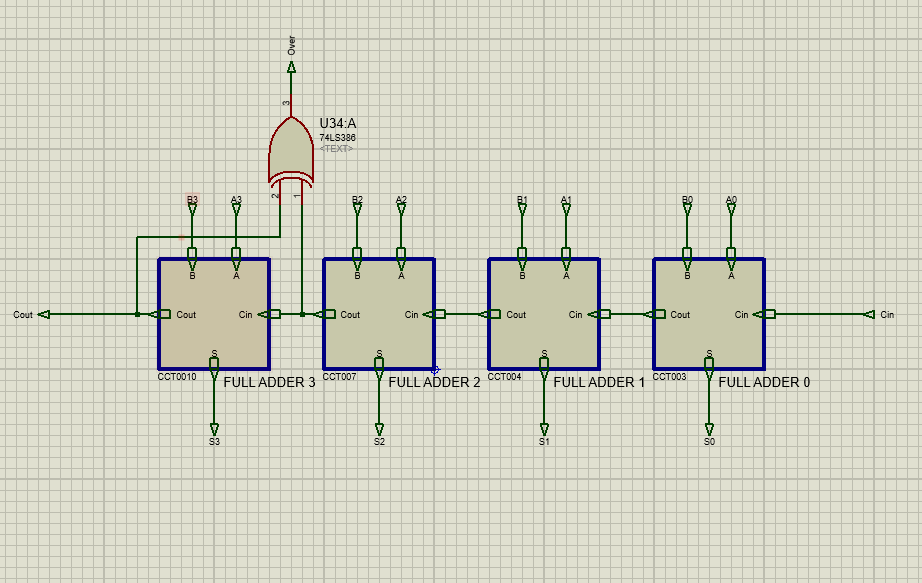
\includegraphics[scale=0.5]{Adder.PNG}
    \caption{Adder}
    \label{fig:Adder}
\end{figure}

\subsubsection{FULL ADDER @}
\begin{figure}[!h]
    \centering
    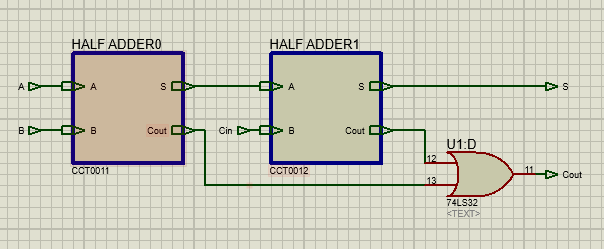
\includegraphics[scale=0.75]{Full-Adder.PNG}
    \caption{Full Adder}
    \label{fig:Full-Adder}
\end{figure}

\subsubsection{HALF ADDER @} 
\begin{figure}[!h]
    \centering
    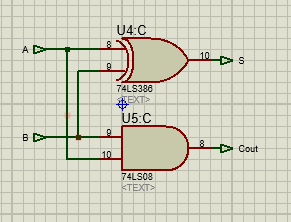
\includegraphics{Half-Adder.PNG}
    \caption{Half Adder}
    \label{fig:Half-Adder}
\end{figure}

\subsubsection{SUBTRACTOR}
\begin{figure}[!h]
    \centering
    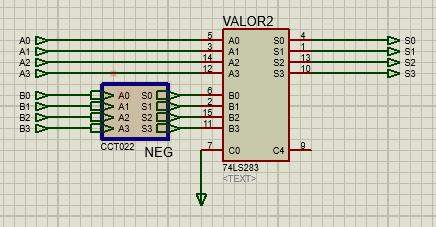
\includegraphics[scale=1]{Subtractor.PNG}
    \caption{Subtractor}
    \label{fig:Subtractor}
\end{figure}

\newpage

\subsubsection{NEG} 
\begin{figure}[h]
    \centering
    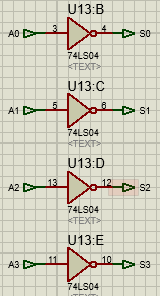
\includegraphics{Neg.PNG}
    \caption{Neg}
    \label{fig:Neg}
\end{figure}

\subsubsection{MUX@} 
\begin{figure}[!h]
    \centering
    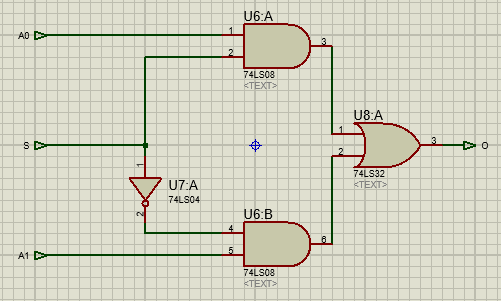
\includegraphics[scale=0.75]{Mux.PNG}
    \caption{Mux}
    \label{fig:Mux}
\end{figure}

\subsubsection{BNNS TO 7SEG @}
\begin{figure}[!h]
    \centering
    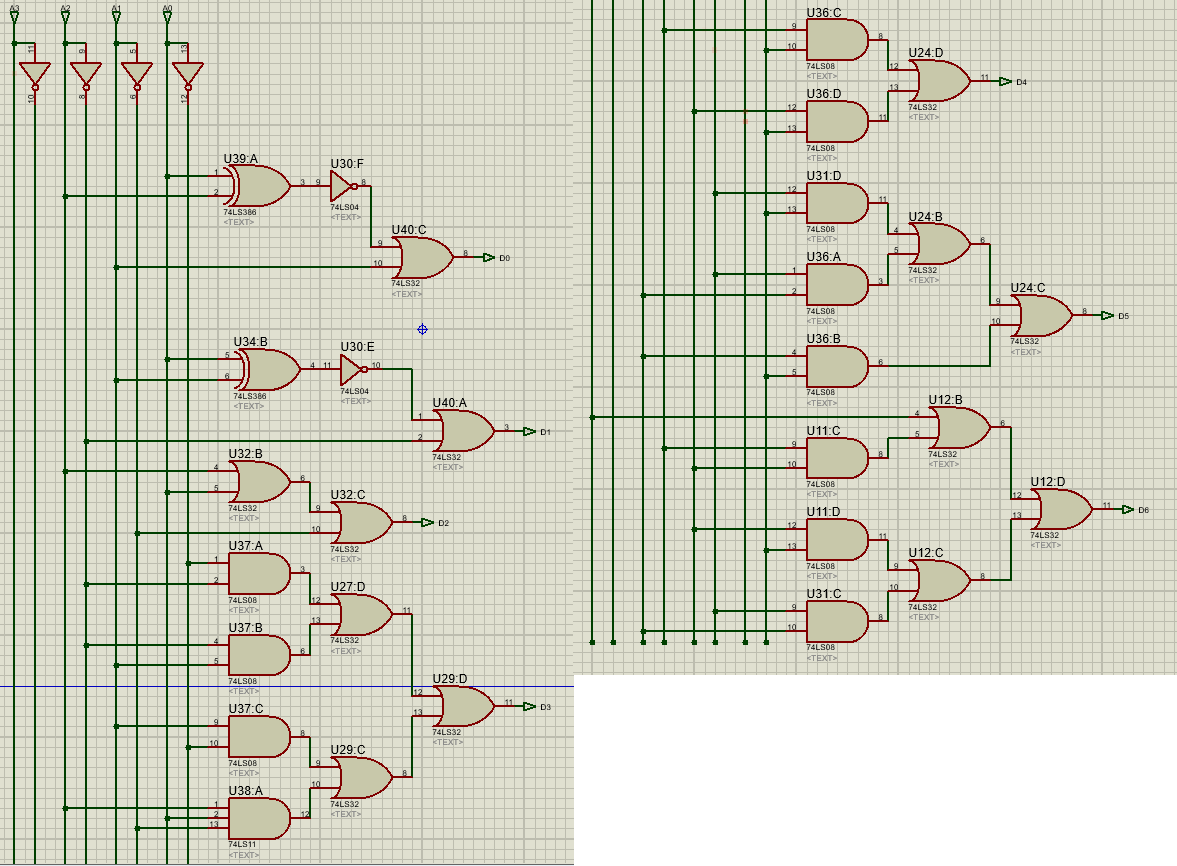
\includegraphics[scale =0.5]{BNSS.PNG}
    \caption{BNNS}
    \label{fig:BNNS}
\end{figure}
\newpage

\subsubsection{ABS C2 TO 7SEG} 
\begin{figure}[!h]
    \centering
    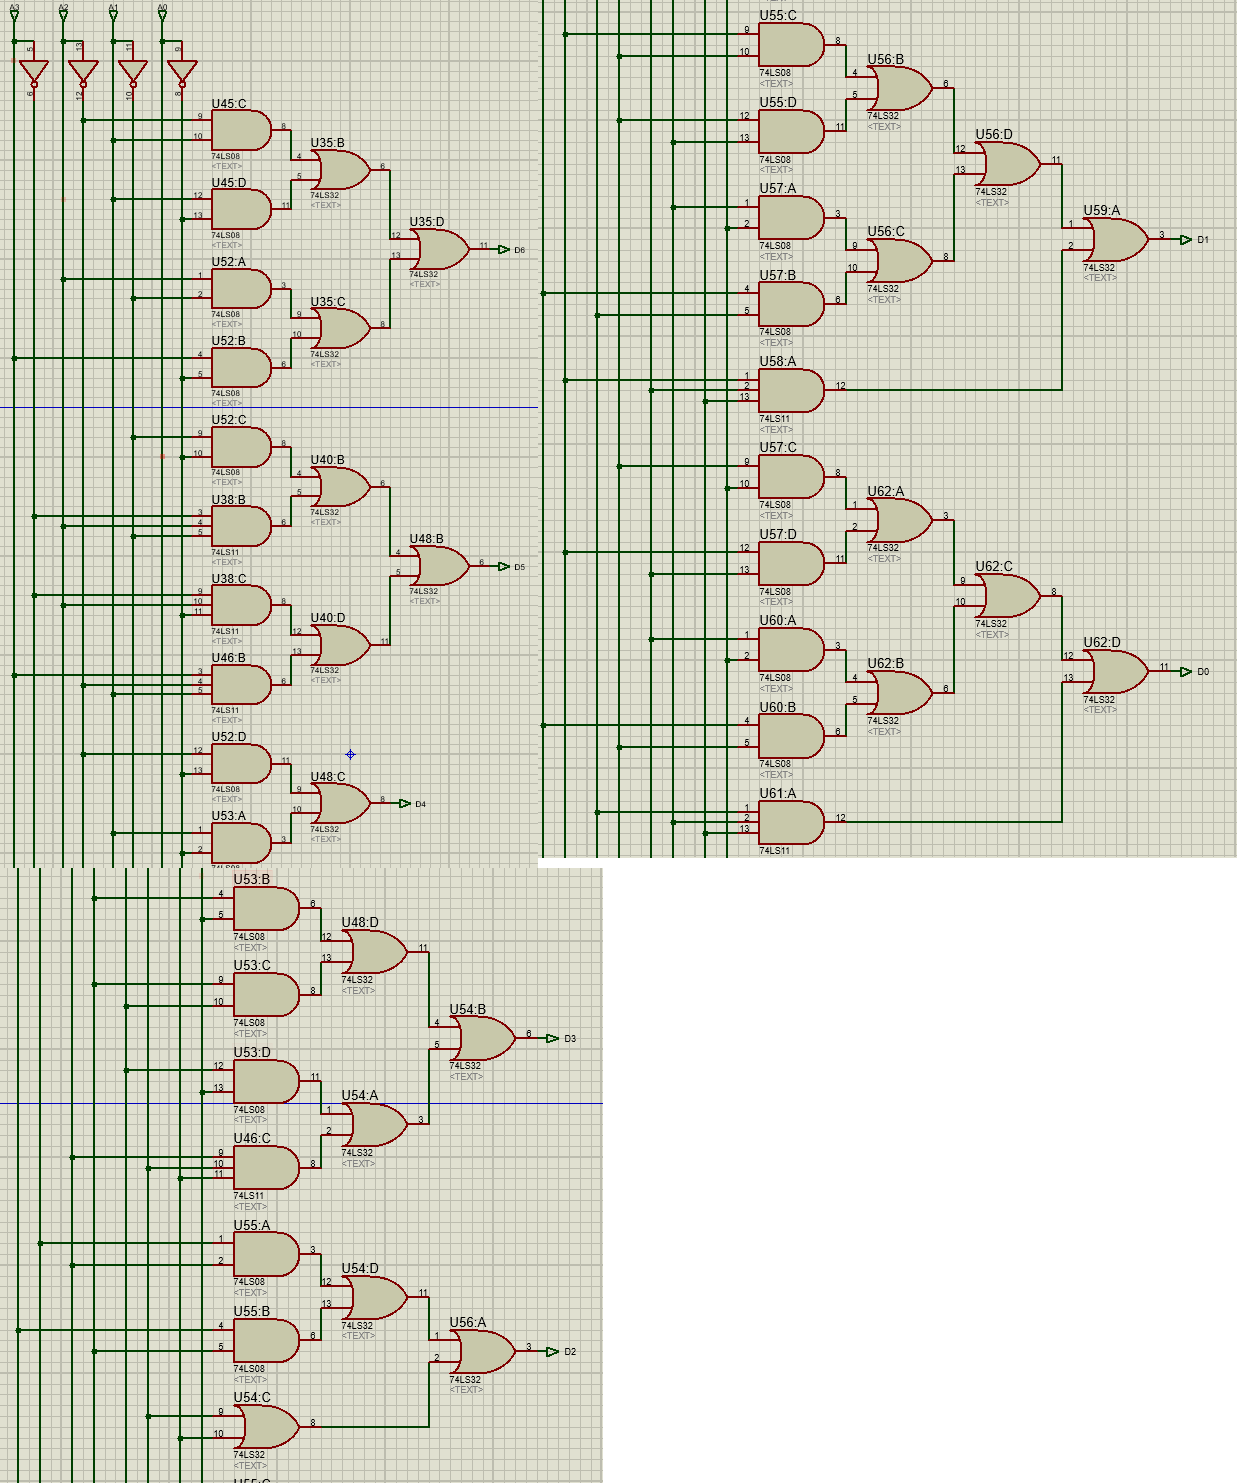
\includegraphics[scale =0.4]{ABS.PNG}
    \caption{ABS}
    \label{fig:ABS}
\end{figure}
\newpage
\subsubsection{EQUALS 0 } 
\begin{figure}[!h]
    \centering
    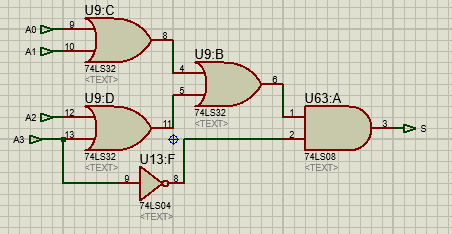
\includegraphics[scale =0.75]{EQUALS.PNG}
    \caption{EQUALS}
    \label{fig:EQUALS}
\end{figure}

\subsubsection{FULL EQUALS}
\begin{figure}[!h]
    \centering
    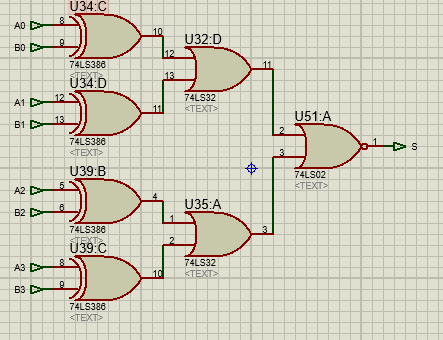
\includegraphics[scale =0.75]{FULLEQUALS.PNG}
    \caption{FULLEQUALS}
    \label{fig:FULLEQUALS}
\end{figure}
\newpage
\subsubsection{B MUX}
\begin{figure}[!h]
    \centering
    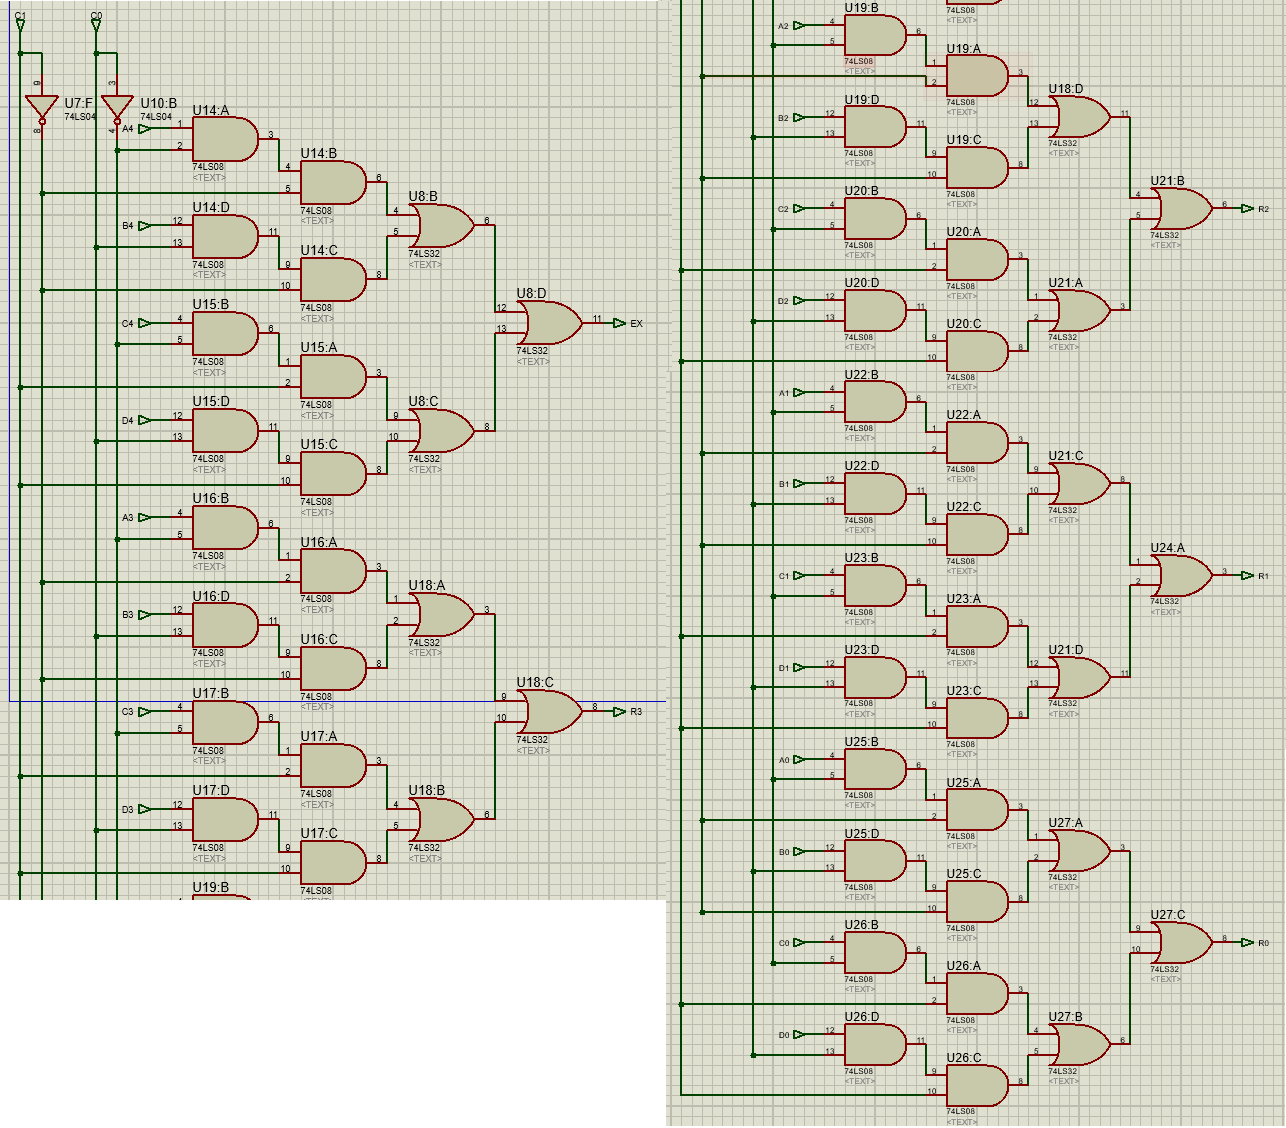
\includegraphics[scale =0.4]{BMUX.PNG}
    \caption{BMUX}
    \label{fig:BMUX}
\end{figure}
\newpage

\subsection{Pruebas realizadas}
Daremos un ejemplo para cada uno de los circuitos y, en el caso que tenga algúna entrada \say{especial} se tomara en cuenta para ver como cambian las salidas. Como valores generales se cogerán -8 para \say{A} y 2 para \say{B} que son, respectivamente, \say{1000} y \say{0010}
\subsubsection{ADDER}
En \say{A} tenemos el valor -8 (1000) y en \say{B} 2 (0010), Cin se mantiene en 0 para todo los casos del circuito. Mediante un conjunto de \hyperref[sec:FULLADDER]{FULL ADDER} se hace la suma de cada uno de los bits de \say{A} y \say{B} individualmente. En este caso \say{S} nos da (1010) que coincide con -6, el resultado que deberia dar. A la hora del display se hizo la decision de representar el valor absoluto de la suma pues el otro display dira si da overflow o no. Para probar que el overflow funciona, podemos tomar el valor 4 tanto para \say{A} como para \say{B}. En este caso, la suma da 1000, que en BNSS representa la salida adecuada. Sin embargo, el valor 8 no se puede representar con 4 bits, el primer display nos representa que hay overflow con una raya horizontal. En el caso que haya overflow, el segundo display, el que representa el valor, es totalmente ignorado.

\subsubsection{FULL ADDER @}
En este caso, no tiene ningun sentido usar -8 y 2 ya que un \hyperref[sec:FULLADDER]{FULL ADDER} solo nos sirve para sumar valores de un solo bit. Si tomamos todas las entradas en 1, \say{A} + \say{B} seria 0, pero como tenemos un carryIn, S seria 1 y Cout seria tambien 1. 

\subsubsection{HALF ADDER @}
El \hyperref[sec:HALFADDER]{HALF ADDER} sigue el mismo camino que el \hyperref[sec:FULLADDER]{FULL ADDER} sin embargo no tiene carry in, esa es la unica diferencia con el FULL ADDER, por lo tanto podemos hacer la misma prueba sin el carryIn. \say{A} + \say{B} seria 0 con un carryOut de 1.

\subsubsection{SUBTRACTOR}
EL \hyperref[sec:SUBTRACTOR]{SUBTRACTOR} se comporta como un \hyperref[sec:ADDER]{ADDER}, sin embargo el carryIn siempre sera 1 y \say{B} estará negado. Para nuestros valores se comportaria, esencialmente como un 1000 + 1101 + 0001 y el resultado nos daria overflow ya que -10 no se puede representar con 4 bits.

\subsubsection{NEG}
No hay mucho que se pueda hacer con \hyperref[sec:NEG]{NEG} ya que simplemente niega todos los bits de la entrada. Si tomamos -8 nos devolveria 0111 y si le damos 2 nos devoleria 1101
\subsubsection{MUX @}
\hyperref[sec:MUX@]{MUX @} Se comportaría como un multiplexor de un solo bit de selección, dependiendo de este bit, la salida será \say{A} o \say{B}.  
\subsubsection{BNSS TO 7SEG @}
\hyperref[sec:BNSS7SEG]{BNSS TO 7SEG} funciona meramente como un codificador para que el display funcione como nosotros queremos, en este caso nos permite decodificar un valor BNSS para que pueda ser representado en un Display. Cabe decir, que solo se tuvieron en cuenta los valores del 0 al 8. Si diesemos -8, el circuito representaria un 8 en el display.
\subsubsection{ABS C2 TO 7SEG}
\hyperref[sec:ABSC27SEG]{ABS C2 TO 7SEG} Es una version mas complicada de \hyperref[sec:BNSS7SEG]{BNSS TO 7SEG} ya que tiene en cuenta el signo. Se decidió usar esta versión del circuito al final para no hacer todo el proceso previo necesario para que BNSS TO 7SEG funcione correctamente. Al igual que su circuito más simple, solo toma valores del 0 al 8. En el caso que dieses -8 el display daria 8.

\subsubsection{EQUALS 0}
Este circuito nos permite identificar si un valor es 0000 o no. Si le pasamos el valor 1000, el circuito nos daria un 0. En cambio, si le damos un 0000 nos devolvera un 1.

\subsubsection{FULL EQUALS}
Este circuito nos permite mirar si dos valores son exactamente iguales. Para ello se hace un recorrido de cada uno de sus bits y mirando si son iguales. Si le pasamos un 1000 y un 0010 el circuito nos devolvera un 0. Si le damos 1110 y 0010 nos seguirá dando 0 aunque los valores absolutos sean iguales. Solo cuando demos dos valores iguales, 1010 y 1010, será cuando el circuito nos devolvera un 1.

\subsubsection{B MUX}
Al igual que \hyperref[sec:MUX@]{MUX @}, dependiendo de unos valores de selección nos permitirá elegir una salida de las 4, en este caso, posibles. Si los bits de seleccion son 00, nos devolverá el valor \say{A}, 01 el \say{B}, 10 el \say{C} y por último 11 el \say{D},

\subsubsection{CIRCUITO}
Para los valores -8 y 2 iremos mirando cuales son todos los posibles resultados del circuito. Para 00 el circuito nos devuelve la suma de -8 y 2, en el display podemos ver el resultado y observamos que no nos da iverflow y el resultado, aunque este en valor absoluto, nos da 6. Probando 4 y 4, observamos que nos da overflow y el resultado da 8. Para 01 nos tiene que devolver el valor absoluto de A, en el caso de -8 el circuito nos devuelve un 8, el segundo display, que nos muestra el valor de EX queda ignorado. Para 10 nos tiene que informar si el valor absoluto de A es mayor que el valor absoluto de B, para el caso de -8 y 2 el circuito nos devuelve un 1 en el valor EX que queda plasmado en el primer display ocmo una barra horizontal. Para 11 nos tiene que informar si A == B, para -8 y 2, el circuito no nos muestra nada. Sin embargo, si cambiamos -8 por 2, vemos que el primer display nos enseña una barra horizontal, dandonos a entender que A == B.
\newpage

\section{Secuencial}

\subsection{Diagrama de estados}
Para que el diagrama fuese mucho más conciso, solo se muestran las entradas que hacen un cambio en el circuito. Es decir, si no se muestra una flecha $\lambda$ de S0 significa que esta formando un lazo consigo mismo.
\begin{figure}[!h]
    \centering
    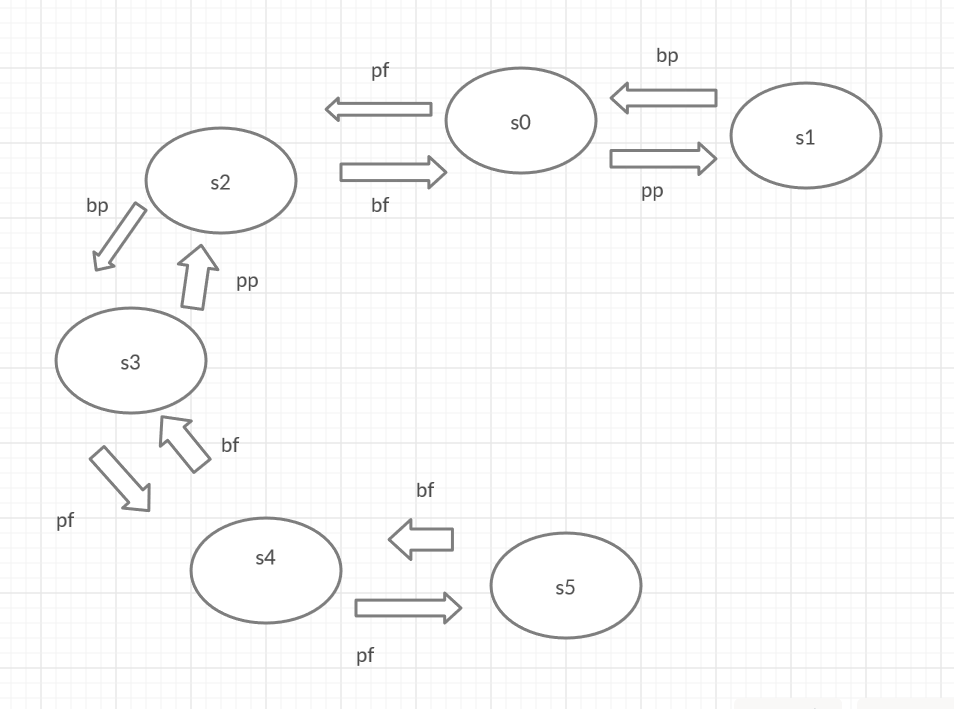
\includegraphics[scale=0.5]{diagrama.PNG}
\end{figure}
\subsection{Codificación de estados}
\begin{multicols}{2}
\noindent Se debe tener en cuenta que necesitamos de 3 bits para codificar nuestras 6 entradas ya que con solo 2 bits solo podemos codificar 4 estados y eso es insuficiente.\vspace{5pt}
    \begin{tabular}{|c|c|}\hline
        qo Totalmente horizontal & 000\\\hline
        q1 Pies elevados frontal horizontal & 001 \\\hline
        q2 Pies horizontal y frontal a nivel 1 & 010 \\\hline
        q3 Pies bajados y frontal a nivel 1 & 011 \\\hline
        q4 Pies bajados y frontal a nivel 2 & 100 \\\hline
        q5 Pies bajados y frontal a nivel 3 & 101 \\\hline
    \end{tabular}

\columnbreak
\noindent Codificamos las 5 entradas en nuestra silla.\vspace{60pt}
\centering
    \begin{tabular}{|c|c|}\hline
        No hacer nada ($\lambda$) & 000\\\hline
        Subir frontal (FP) & 001 \\\hline
        Bajar frontal (FB) & 010 \\\hline
        Subir pies (PP) & 011 \\\hline
        Bajar pies (PB) & 100 \\\hline
    \end{tabular}
\end{multicols}
\subsection{Justificación del tipo de máquina}
Para la parte secuencial de nuestro trabajo usaremos una máquina de tipo Mealy puesto que al tener que representar cómo funciona una silla, esta depende del estado actual y de la entrada en la que se encuentre.

Esto se ve claramente con el siguiente caso; Si estamos en el estado q2 ( pies horizontales y frontal a nivel 1) y nos entra un subir frontal, no haremos nada puesto que no existe el estado pies horizontal y frontal a nivel 2.
\newpage
\subsection{Tabla de trasición} 
\begin{figure}[!h]
    \centering
    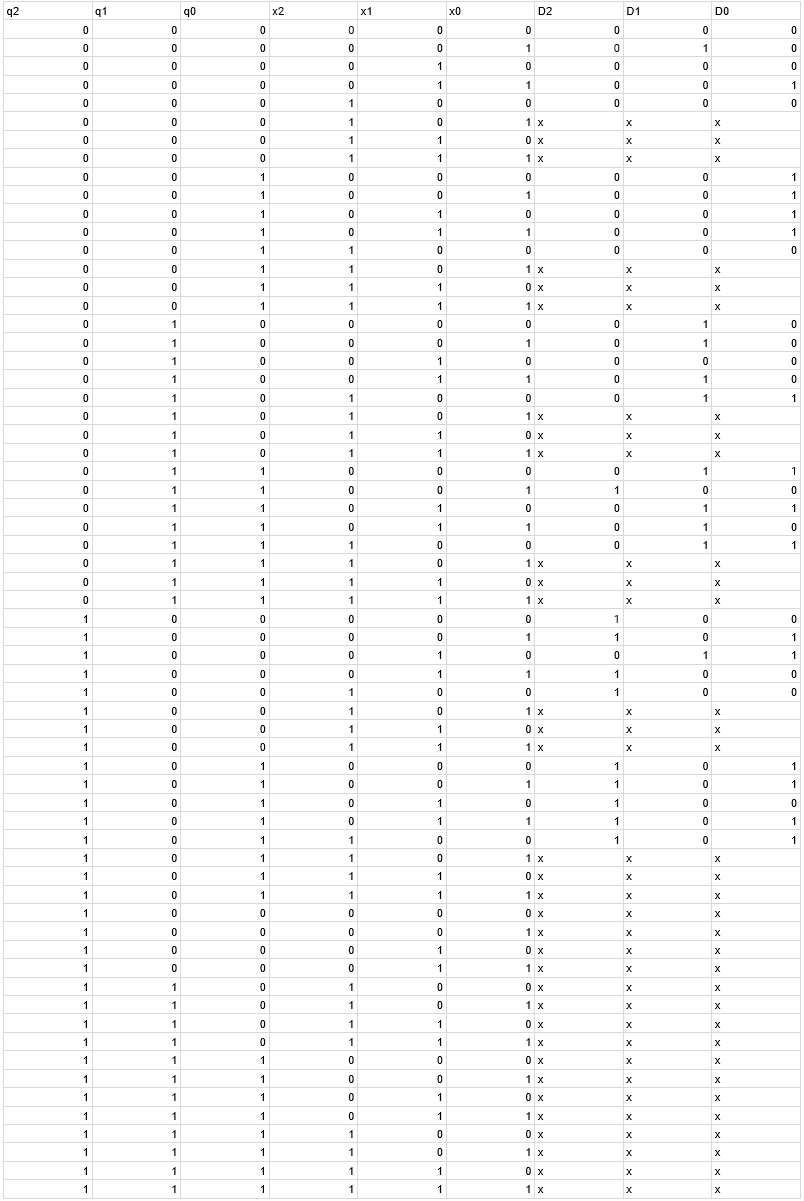
\includegraphics[scale=0.73]{TABLA.PNG}
\end{figure}
\subsection{Minimización}
Como los Flip-Flop son de tipo D, podemos coger el estado siguiente (qy') como nuestro valor para cada uno de nuestros Flip-Flop. De esta manera obtenemos las funciones:
\setlist[description]{font=\normalfont\textbullet\space}
\begin{description}
    \item[D1: ]$Y=BD + AC\overline{E} + A\overline{E}F + \overline{B}CF + \overline{A}C\overline{D}\overline{F} + \overline{A}\overline{B}EF + A\overline{C}E\overline{F}$
    \item[D2: ]$Y=B\overline{C}\overline{E} + BEF + BC\overline{F} + \overline{A}\overline{C}\overline{E}F + A\overline{C}E\overline{F}$
    \item[D3: ]$Y=A\overline{B} + AF + AC + BC\overline{E}F$
\end{description}
\subsection{Implementación}
En orden de completar esta práctica hemos tenido que implementar todo el material anterior (tablas de verdad, karnaugh..) usando proteus de la manera siguiente:\\

Presentamos nuestro programa con 4 Logic Toggles que simbolizan los 4 botones que tiene
el mando de la silla que se nos ha mandado programar, estas 4 entradas se transforman en
3 bits siguiendo un simple mapa de karnaugh hecho teniendo mente el hecho de que según
nuestra codificación el botón FP se traducirá en 001 y así con el resto de botones.

\begin{figure}[!h]
    \centering
    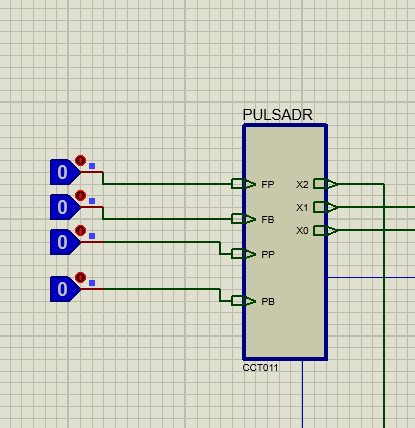
\includegraphics{COMMENT3.PNG}
\end{figure}
Luego, siguiendo los mapas de karnaugh obtenidos anteriormente hemos creado nuestros
Flip/Flops de tipo D, estas implementaciones de los mapas de karnaugh están ocultos en
hojas hijas para mejorar la legibilidad de nuestro programa, cabe destacar la
retroalimentación de las entradas que caracteriza a los sistemas secuenciales, recordemos
también que necesitamos 3 Flip/Flops de clase D ya que tenemos 3 bits para codificar los
estados.

\begin{figure}[!h]
    \centering
    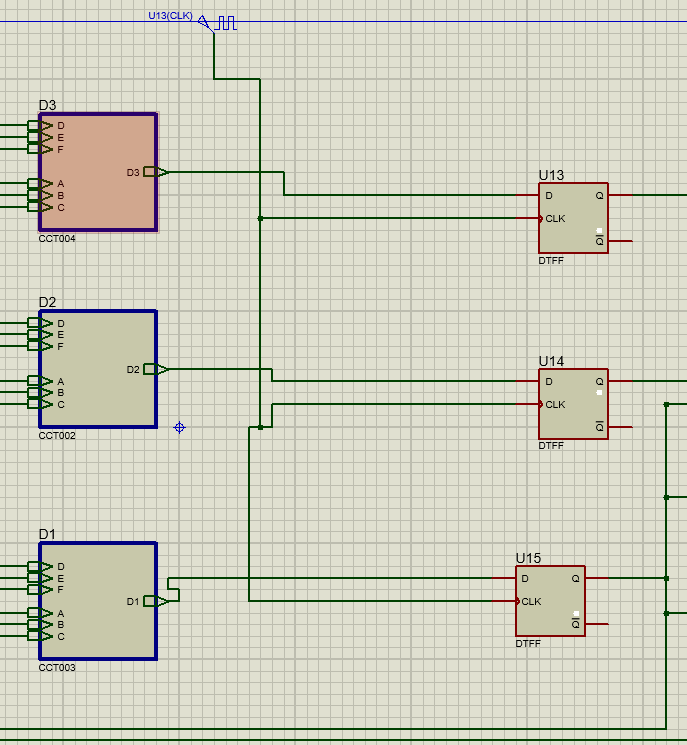
\includegraphics[scale=0.5]{COMMENT1.PNG}
\end{figure}

\newpage
El resultado de este programa se puede entender como la visualización de la silla según los
estados que se accionen en nuestros Logic States, para lograr esto hemos tenido que
codificar mediante mapas de karnaugh las diferentes partes de los Displays, un ejemplo de
esto sería si las 3 d’ s son 000 (estado codificado anteriormente) se debe visualizar la silla
totalmente horizontal, como en la parte anterior hemos decidido ocultar los circuitos que
codifican dichas visualizaciones en hojas hijas para mayor comodidad.

\begin{figure}[!h]
    \centering
    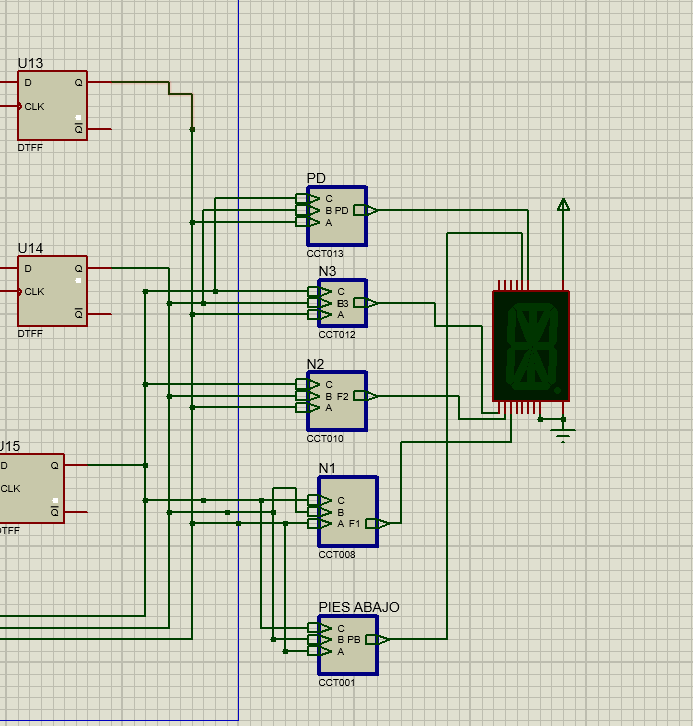
\includegraphics[scale=0.5]{COMMENT2.PNG}
\end{figure}
\newpage
\subsection{Juego de pruebas y cronograma de las salidas para un ejemplo}
Recordemos que por teoría hemos visto que usando un flip flop de clase D, este solo puede cambiar en el momento en el que el clock vale 1, así pues vemos como nuestras capturas cumplen dicha condición. En este caso, la linea amarilla representa nuestro clock.

\begin{figure}[!h]
    \centering
    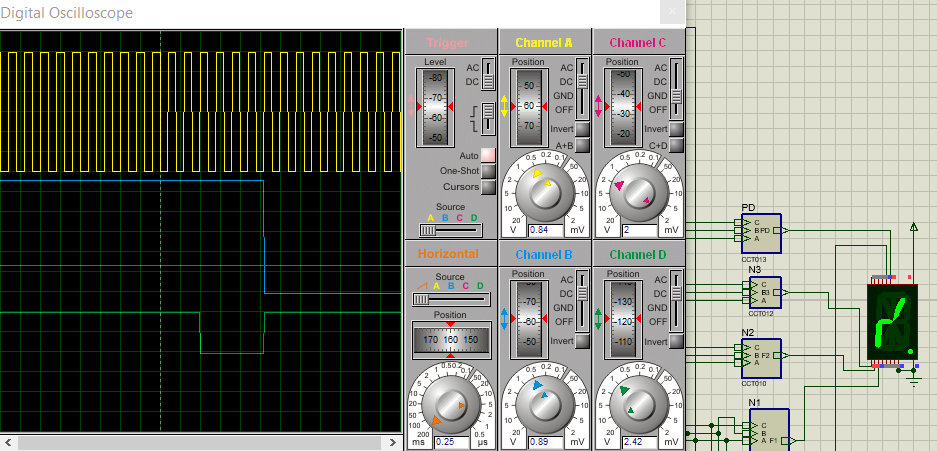
\includegraphics[scale=0.5]{1.PNG}
\end{figure} 

\begin{figure}[!h]
    \centering
    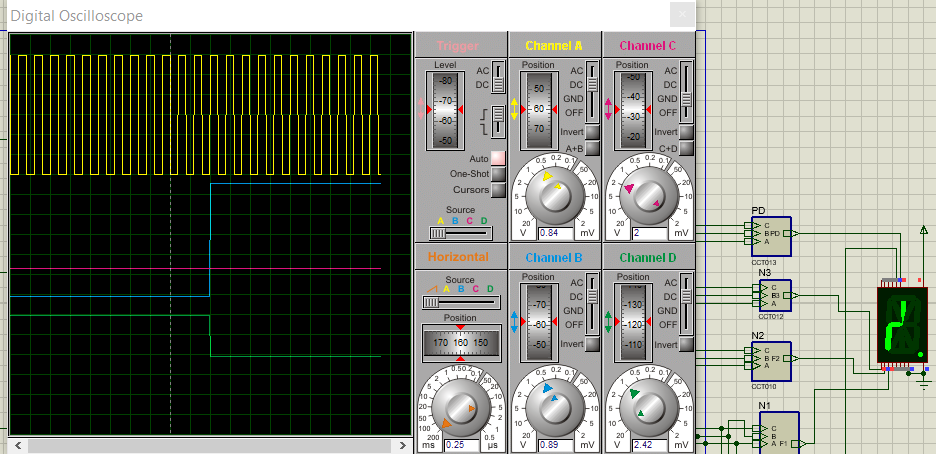
\includegraphics[scale=0.5]{4.PNG}
\end{figure}

\newpage
\section{Conclusiones}
Durante todo el desarrollo de este proyecto hemos adquirido una gran canitad de conocimiento y sobre todo habilidad de movimiento dentro de Proteus. Aunque hayamos tenido problemas en algunos puntos contados, en conjunto creemos que la practica ha sido una gran oportunidad para ponerte a prueba y ver cuan bien puedes hacerlo.\\

Cabe mencionar que no todo fue proteus, sino tambien optimización de tiempo, esfuerzo y funciones lógicas. Hemos tenido que lidiar con la manera de pensar del otro para que nuestros circuitos sean faciles de leer entre autores y poder sacar el mejor circuito que nos agradase a los dos a la vez.\\

Ademas, ha sido una buena oportunidad para ver y usar un sistema de versiones como Github, donde se fue documentando cada versión. Y por parte de la memoria, el uso de \LaTeX  lo que nos obligo a hacer una memoria a parte a \say{sucio} y luego pasarla a un formato más agradable.\\

En conjunto, ha sido una experiencia que nos ha puesto a prueba y sobre todo nos a ayudado a ver como funcionan este tipo de trabajos.
\end{document}
%Y asi, yo muero y lo dejo todo a mi gato guantes. Vive una buena vida
%me cago en tu vida marc